\documentclass[10pt]{extarticle} 
\usepackage{unicode-math}
\usepackage{mathrsfs}
\usepackage{amsthm,graphicx,xcolor,natbib,enumitem,booktabs,tabularx}
\usepackage[paperwidth=126mm, paperheight=96mm, top=5mm, bottom=5mm, right=5mm, left=5mm]{geometry}
\pagenumbering{gobble}

\usepackage[BoldFont,SlantFont]{xeCJK}  
\xeCJKsetemboldenfactor{2}
%\setCJKmainfont{cwTeX Q Kai Medium}
%\setCJKmainfont{cwTeX Q Ming Medium}
\setCJKmainfont{cwTeX Q Yuan Medium}
%\usepackage[AutoFakeBold,AutoFakeSlant]{xeCJK}  
%\setCJKmainfont[AutoFakeSlant=.1,AutoFakeBold=1]{cwTeX Q Kai Medium} 
%\setCJKfamilyfont{kaiv}[Vertical=RotatedGlyphs]{cwTeX Q Medium}
%\setmainfont{texgyrepagella-regular.otf}
%\setmathfont{texgyrepagella-math.otf}

\usepackage{hyperref}
\hypersetup{
    colorlinks,
    linkcolor={red!50!black},
    citecolor={blue!60!black},
    urlcolor={blue!60!black}
    %urlcolor={blue!80!black}
}

\newcommand{\ds}{\displaystyle}
\newcommand{\ie}{\;\Longrightarrow\;}
\newcommand{\ifff}{\;\Longleftrightarrow\;}
\newcommand{\orr}{\;\vee\;}
\newcommand{\andd}{\;\wedge\;}
\newcommand{\mi}{\mathrm{i}}
\newcommand{\llt}{\left\langle}
\newcommand{\rgt}{\right\rangle}
\DeclareMathOperator*{\dom}{dom}
\DeclareMathOperator*{\codom}{codom}
\DeclareMathOperator*{\ran}{ran}
\DeclareMathOperator*{\sgn}{sgn}
\DeclareMathOperator*{\degr}{deg}
\DeclareMathOperator*{\jac}{D}
\newcommand{\floor}[1]{\lfloor #1 \rfloor}
\newcommand{\ceil}[1]{\lceil #1 \rceil}
\newcommand{\proj}[2]{\mathrm{proj}_{\,#2}\,#1}

\DeclareMathOperator*{\argmax}{\arg\!\max}
\DeclareMathOperator*{\argmin}{\arg\!\min}
\DeclareMathOperator*{\im}{Im}
\DeclareMathOperator*{\re}{Re}

\theoremstyle{definition}
\newtheorem*{dfn}{Definition}
\newtheorem*{prp}{Property}
\newtheorem*{thm}{Theorem}
\newtheorem*{ex}{Example}
\newtheorem*{sol}{Solution}
\newtheorem*{prf}{Proof}
\newtheorem*{fact}{Fact}
\newtheorem*{rmk}{Remark}

\usepackage{multicol}

%%%%%%%%%%%%%%%%%%%%%%%%%%%%%%%%%%%%%%%%%%%%%%%%%%%%%%%%%%%%%
% from clp3

\newcommand{\vr}{\mathbf{r}}
\newcommand{\vR}{\mathbf{R}}
\newcommand{\va}{\mathbf{a}}
\newcommand{\vb}{\mathbf{b}}
\newcommand{\vc}{\mathbf{c}}
\newcommand{\vd}{\mathbf{d}}
\newcommand{\ve}{\mathbf{e}}
\newcommand{\vC}{\mathbf{C}}
\newcommand{\vp}{\mathbf{p}}
\newcommand{\vn}{\mathbf{n}}
\newcommand{\vu}{\mathbf{u}}
\newcommand{\vv}{\mathbf{v}}
\newcommand{\vV}{\mathbf{V}}
\newcommand{\vx}{\mathbf{x}}
\newcommand{\vX}{\mathbf{X}}
\newcommand{\vy}{\mathbf{y}}
\newcommand{\vz}{\mathbf{z}}
\newcommand{\vf}{\mathbf{f}}
\newcommand{\vF}{\mathbf{F}}
\newcommand{\vg}{\mathbf{g}}
\newcommand{\vG}{\mathbf{G}}
\newcommand{\vH}{\mathbf{H}}
\newcommand{\vM}{\mathbf{M}}
\newcommand{\vT}{\mathbf{T}}
\newcommand{\vN}{\mathbf{N}}
\newcommand{\vL}{\mathbf{L}}
\newcommand{\vA}{\mathbf{A}}
\newcommand{\vB}{\mathbf{B}}
\newcommand{\vD}{\mathbf{D}}
\newcommand{\vE}{\mathbf{E}}
\newcommand{\vJ}{\mathbf{J}}
\newcommand{\vZero}{\mathbf{0}}
\newcommand{\vPhi}{\mathbf{\Phi}}
\newcommand{\vOmega}{\mathbf{\Omega}}
\newcommand{\vTheta}{\mathbf{\Theta}}
\newcommand{\cA}{\mathcal{A}}
\newcommand{\cB}{\mathcal{B}}
\newcommand{\cM}{\mathcal{M}}
\newcommand{\cO}{\mathcal{O}}
\newcommand{\cR}{\mathcal{R}}
\newcommand{\cS}{\mathcal{S}}
\newcommand{\cT}{\mathcal{T}}
\newcommand{\cU}{\mathcal{U}}
\newcommand{\cV}{\mathcal{V}}
\newcommand{\cW}{\mathcal{W}}
\newcommand{\cX}{\mathcal{X}}
%\newcommand{\hi}{\hat{\mathbf{i}}}
%\newcommand{\hj}{\hat{\mathbf{j}}}
\newcommand{\hi}{\widehat{\pmb{\imath}}}
\newcommand{\hj}{\widehat{\pmb{\jmath}}}
\newcommand{\hk}{\widehat{\mathbf{k}}}
\newcommand{\hn}{\widehat{\mathbf{n}}}
\newcommand{\hr}{\widehat{\mathbf{r}}}
\newcommand{\hvt}{\widehat{\mathbf{t}}}
\newcommand{\hN}{\widehat{\mathbf{N}}}
\newcommand{\vth}{{\pmb{\theta}}}
\newcommand{\vTh}{{\pmb{\Theta}}}
%\newcommand{\vnabla}{\pmb{\nabla}}
\newcommand{\vnabla}{   { \mathchoice{\pmb{\nabla}}
                            {\pmb{\nabla}}
                            {\pmb{\scriptstyle\nabla}}
                            {\pmb{\scriptscriptstyle\nabla}} }   }
\newcommand{\ha}[1]{\mathbf{\hat e}^{(#1)}}

\newcommand{\bbbc}{\mathbb{C}}

\newcommand{\Om}{\Omega}
\newcommand{\om}{\omega}
\newcommand{\vOm}{\pmb{\Omega}}
\newcommand{\svOm}{\pmb{\scriptsize\Omega}}
\newcommand{\al}{\alpha}
\newcommand{\be}{\beta}
\newcommand{\de}{\delta}
\newcommand{\ga}{\gamma}
\newcommand{\ka}{\kappa}
\newcommand{\la}{\lambda}

\newcommand{\cC}{\mathcal{C}}
\newcommand{\bbbone}{\mathbb{1}}

\def\tr{\mathop{\rm tr}}
\newcommand{\Atop}[2]{\genfrac{}{}{0pt}{}{#1}{#2}}

%\newcommand{\pdiff}[2]{ \frac{\partial\hfil#1\hfil}{\partial #2}}
\newcommand{\pdiff}[2]{\frac{\partial #1}{\partial #2}}
\newcommand{\pdifft}[2]{\frac{\partial^2 #1}{\partial #2^2}}
\newcommand{\dblInt}{\iint}
\newcommand{\tripInt}{\iiint}
%\newcommand{\dblInt}{\int\!\!\int}
%\newcommand{\tripInt}{\int\!\!\!\int\!\!\!\int}
%\newcommand{\dblInt}{\mathop{\int\!\!\!\int}}
%\newcommand{\tripInt}{\mathop{\int\!\!\!\int\!\!\!\int}}

\newcommand{\Set}[2]{\big\{ \ #1\ \big|\ #2\ \big\}}
\newcommand{\rhof}{{\rho_{\!{\scriptscriptstyle f}}}}
\newcommand{\rhob}{{\rho_{{\scriptscriptstyle b}}}}

\renewcommand{\neg}{ {\sim} }
\newcommand{\limp}{ {\;\Rightarrow\;} }
\newcommand{\nimp}{ {\;\not\Rightarrow\;} }
\newcommand{\liff}{ {\;\Leftrightarrow\;} }
\newcommand{\niff}{ {\;\not\Leftrightarrow\;} }

\newcommand{\st}{ {\mbox{ s.t. }} }
\newcommand{\es}{ {\varnothing}}
\newcommand{\pow}[1]{ \mathcal{P}\left(#1\right) }
\newcommand{\set}[1]{ \left\{#1\right\} }

\newcommand{\bbbn}{\mathbb{N}}
\newcommand{\bbbr}{\mathbb{R}}
\newcommand{\bbbp}{\mathbb{P}}
\newcommand{\De}{\Delta}
\newcommand{\cD}{\mathcal{D}}
\newcommand{\cP}{\mathcal{P}}
\newcommand{\cI}{\mathcal{I}}
\newcommand{\veps}{\varepsilon}
\newcommand{\dee}[1]{\mathrm{d}#1}

\newcommand{\bdiff}[2]{ \frac{\mathrm{d}}{\mathrm{d}#2} \left( #1 \right)}
\newcommand{\ddiff}[3]{ \frac{\mathrm{d}^#1#2}{\mathrm{d}{#3}^#1}}
\newcommand{\half}{\tfrac{1}{2}}
\newcommand{\diff}[2]{\frac{\mathrm{d} #1}{\mathrm{d} #2}}
\newcommand{\difftwo}[2]{\frac{\mathrm{d^2} #1}{\mathrm{d}{#2}^2}}

%%%%%%%%%%%%%%%%%%%%%%%%%%%%%%%%%%%%%%%%%%%%%%%%%%%%%%%%%%%%%%%%%%%%%

\newcommand\scalemath[2]{\scalebox{#1}{\mbox{\ensuremath{\displaystyle #2}}}}

\begin{document}
\title{\texorpdfstring{\vspace{15mm} Operations Research\\ 04. Optimization Fundamentals}{Operations Research\\ 04. Optimization Fundamentals}} 
\author{}
\date{}
\maketitle
\newpage

%https://www.youtube.com/shorts/wlffDYJC0Z4?feature=share

\section*{The Chain Rule}
\begin{dfn}[The Jacobian]
  Let $V$ be open in $\mathbb{R}^n$, $\vx\in V$, and $g_i:V\to\mathbb{R}$, $i = 1,\,2,\,\ldots,\,m$ be $C^1$ on $V$. The Jacobian of $\vg(\vx): \mathbb{R}^n\to\mathbb{R}^m$ is defined as
  \begin{align*}
    \jac\vg(\vx) = %\frac{\partial(g_1,\,g_2,\,\ldots,\,g_m)}{\partial (x_1,\,x_2,\,\ldots,\,x_{\!n})}(\vx) = 
    \begin{pmatrix}
      \frac{\partial g_1}{\partial x_1} & \frac{\partial g_1}{\partial x_2} & \cdots & \frac{\partial g_1}{\partial x_{\!n}} \\
      \frac{\partial g_2}{\partial x_1} & \frac{\partial g_2}{\partial x_2} & \cdots & \frac{\partial g_2}{\partial x_{\!n}} \\
      \vdots & \vdots & \ddots &\vdots \\
      \frac{\partial g_m}{\partial x_1} & \frac{\partial g_m}{\partial x_2} & \cdots & \frac{\partial g_m}{\partial x_{\!n}}
    \end{pmatrix}(\vx)
  \end{align*}
\end{dfn}
\begin{thm}[\citet{rudin} 9.15; \citet{apostol_adv} Theorem 12.7; \citet{wade} 11.28]
  Suppose that $\vf$ and $\vg$ are vector functions. If $\vg$ is differentiable at $\va$ and $\vf$ is differentiable at $\vg(\va)$, then $\vf\circ\vg$ is differentiable at $\va$ and
  \begin{align*}
    \jac(\vf\circ\vg)(\va) = \jac\vf(\vg(\va))\,\jac\vg(\va)
  \end{align*}
  More explicitly, if $f$ is a differentiable function of $x_1,\,x_2,\,\ldots,\,x_n$, and each $x_j$ is a differentiable function of $t_1,\,t_2,\,\ldots,\,t_m$, $n$, $m\geqslant 1$; then $f$ is a differentiable function of $t_1,\,t_2,\,\ldots,\,t_m$ with
  \begin{align*}
    \pdiff{f}{t_i} = \pdiff{f}{x_1}\,\pdiff{x_1}{t_i} + \pdiff{f}{x_2}\,\pdiff{x_2}{t_i} + \cdots + \pdiff{f}{x_n}\,\pdiff{x_n}{t_i}
  \end{align*}
\end{thm}

\newpage

\begin{ex}
  Let $w = f(x z, y z)$, where $f$ is a differentiable function. Prove that $\ds x\frac{\partial w}{\partial x} + y\frac{\partial w}{\partial y} = z\frac{\partial w}{\partial z}$.
\end{ex}

\begin{sol}
  Write $u(x,y,z)=xz$ and $v(x,y,z)=yz$ so that $w(x,y,z) = f\big(u(x,y,z), v(x,y,z)\big)$. By the chain rule,
  \begin{align*}
    &\pdiff{w}{x}(x,y,z) = \pdiff{}{x}\big[f \big(u(x,y,z), v(x,y,z)\big)\big] \\
    &= \pdiff{f}{u}\big(u(x,y,z), v(x,y,z)\big)\pdiff{u}{x}(x,y,z) + \pdiff{f}{v}\big(u(x,y,z), v(x,y,z)\big)\pdiff{v}{x}(x,y,z) \\ 
    &= z\pdiff{f}{u}(xz, yz)
  \end{align*}
  \begin{align*}
    &\pdiff{w}{y}(x,y,z) = \pdiff{}{y}\big[f \big(u(x,y,z), v(x,y,z)\big)\big] \\
    &= \pdiff{f}{u}\big(u(x,y,z), v(x,y,z)\big)\pdiff{u}{y}(x,y,z) + \pdiff{f}{v}\big(u(x,y,z), v(x,y,z)\big)\pdiff{v}{y}(x,y,z) \\
    &= z\pdiff{f}{v}(xz, yz)
  \end{align*}
  \begin{align*}
    &\pdiff{w}{z}(x,y,z) = \pdiff{}{z}\big[f \big(u(x,y,z), v(x,y,z)\big)\big] \\
    &= \pdiff{f}{u}\big(u(x,y,z), v(x,y,z)\big)\pdiff{u}{z}(x,y,z) + \pdiff{f}{v}\big(u(x,y,z), v(x,y,z)\big)\pdiff{v}{z}(x,y,z) \\
    &= x\pdiff{f}{u}(xz, yz) + y\pdiff{f}{v}(xz, yz)
  \end{align*}
  So
  \begin{align*}
    \pdiff{w}{x} + y\pdiff{w}{y} &= xz\pdiff{f}{u}(xz, yz) + yz\pdiff{f}{v}(xz, yz) \\&= z\left[x\pdiff{f}{u}(xz, yz) + y\pdiff{f}{v}(xz, yz)\right] = z\pdiff{w}{z}
  \end{align*}
\end{sol}

\newpage
\section*{Unconstrained Optimization Problems}

\begin{thm}[\citet{rudin} 4.16; \citet{apostol_adv} Theorem 4.27; \citet{wade} 9.57]
  Given $\ds S\subseteq\mathbb{R}^n$ and continuous $f: S\to\mathbb{R}$; if $S$ is compact, then  
  \begin{align*}
    M = \sup\left\{f(\vx): \vx\in S\right\}\quad\text{ and }\quad m = \inf\left\{f(\vx): \vx\in S\right\}
  \end{align*}
  are finite real numbers. Moreover, there exists points $\vx_\text{M}$, $\vx_\text{m}\in S$ such that $M = f(\vx_\text{M})$ and $m = f(\vx_\text{m})$.
\end{thm}

\begin{dfn}
  Given $\ds S\subseteq\mathbb{R}^n$, $\ds f:S\to\mathbb{R}$ and $\ds B(\vx, h)\equiv\{\vy\in\mathbb{R}^n\;|\;|\vy - \vx| < h\}$, $f$ achieves 
  \begin{itemize}%\setlength\itemsep{0em}
    \item global maximum $\ds f(\vx_\text{M})$ at $\ds\vx_\text{M}\in S$: $\ds f(\vx_\text{M})\geqslant f(\vx),\;\forall\,\vx\in S$. 
    \item global minimum $\ds f(\vx_\text{m})$ at $\ds \vx_\text{m}\in S$: $\ds f(\vx_\text{m})\leqslant f(\vx),\;\forall\,\vx\in S$. 
    \item local maximum $\ds f(\vx_0)$ at $\ds\vx_0\in S$: $\ds\exists\,h_0 > 0$ s.t. $\ds f(\vx_0)\geqslant f(\vx),\;\forall\,\vx\in B(\vx_0, h_0)\,\cap\,S$. 
    \item local minimum $\ds f(\vx_1)$ at $\ds\vx_1\in S$: $\ds\exists\,h_1 > 0$ s.t. $\ds f(\vx_1)\leqslant f(\vx),\;\forall\,\vx\in B(\vx_1, h_1)\,\cap\,S$. 
  \end{itemize}
\end{dfn}

\newpage

\begin{thm}[necessary conditions for extremum]
  Given $\ds S\subseteq\mathbb{R}^n$ and differentiable $\ds f:S\to\mathbb{R}$, if $f$ achieves extremum at an interior $\vc\in S$, then $\ds\nabla f(\vc) = \vZero$. 
\end{thm}

\begin{prf}
  If $\ds\vc = (c_1,\,c_2,\,\ldots,\,c_n)$, let 
  \begin{align*}
    g_j(t)\equiv f(c_1,\,c_2,\,\ldots,\,c_{j - 1},\,t,\,c_{j + 1},\,\ldots,\,c_n), \quad j = 1,\,2,\,\ldots,\,n 
  \end{align*}
  For $f$ achieves extremum at $\vc$, $f(\vc) = g_j(c_j)$, $g_j$ achieves extremum at $c_j\ie g_j'(t)\,\big|_{t = c_j} = 0 \ie D_j f(\vc) = 0\;\forall\,j$, so $\ds\nabla f(\vc) = \vZero$.  
\end{prf}

\begin{thm}
  Given $\ds S\subseteq\mathbb{R}^n$, if $f:S\to\mathbb{R}$ achieves extremum at $\vc\in S$, then $\vc$ can possibly be a
    \begin{itemize}%\setlength\itemsep{0em}
      \item critical point: $\ds \nabla f(\vc) = \vZero$. 
      \item singular point: $f$ is non-differentiable at $\vc$.  
      \item boundary point of $S$. 
    \end{itemize}
\end{thm}

\newpage

%\section*{Multivariable Differential Calculus}
%\subsection*{The Directional Derivatives}
%\subsection*{The Total Derivative}
%\subsection*{The Total Derivative Expressed in Terms of Partial Derivatives}
%\subsection*{The Matrix of a Linear Function}
%\subsection*{The Jacobian Matrix}
%\subsection*{The Mean-Value Theorem for Differentiable Functions}
%\subsection*{Taylor's Formula for Functions from $\mathbb{R}^n$ to $\mathbb{R}^1$}

\begin{dfn}[Hessian Matrix]
  Given $\ds S\subseteq\mathbb{R}^n$, an interior point $\vc$ of $S$, and a differentiable function $\ds f:S\to\mathbb{R}$, 
  \begin{align*}
    \vH(f, \vc) = \begin{pmatrix}f_{11} & f_{12} & \cdots & f_{1n} \\ f_{21} & f_{22} & \cdots & f_{2n} \\ \vdots & \vdots & \ddots & \vdots \\ f_{n1} & f_{n2} & \cdots & f_{nn}\end{pmatrix}, \quad f_{ij} = \frac{\partial^2 f}{\partial x_j\partial x_i}(\vc), \quad i,\,j = 1,\,2,\,\ldots,\,n.
  \end{align*}
\end{dfn}

\begin{dfn}[Matrix Positive/Negative Definiteness] 
  Given an $n\times n$ real symmetric matrix $\vA$. For any $\ds\vv\in\mathbb{R}^n\ne\vZero$, $\vA$ is
  \begin{itemize}%\setlength\itemsep{0em}
    \item positive-definite: $\ds\vv\vA\vv^\top > 0$ 
    \item negative-definite: $\ds\vv\vA\vv^\top < 0$
    \item positive-semidefinite: $\ds\vv\vA\vv^\top\geqslant 0$
    \item negative-semidefinite: $\ds\vv\vA\vv^\top\leqslant 0$
  \end{itemize}
\end{dfn}

\begin{dfn}[Minor] 
  Given an $n\times n$ matrix $\ds\vA = \begin{pmatrix}a_{11} & a_{12} & \cdots & a_{1n} \\ a_{21} & a_{22} & \cdots & a_{2n} \\ \vdots & \vdots & \ddots & \vdots \\ a_{n1} & a_{n2} & \cdots & a_{nn} \end{pmatrix}$ and minor $\ds\vA\begin{pmatrix}i_1,\,i_2,\,\cdots,\,i_k\\j_1,\,j_2,\,\cdots,\,j_k\end{pmatrix} = \begin{vmatrix}a_{i_1 j_1} & a_{i_1 j_2} & \cdots & a_{i_1 j_k} \\ a_{i_2 j_1} & a_{i_2 j_2} & \cdots & a_{i_2 j_k} \\ \vdots & \vdots & \ddots & \vdots \\ a_{i_k j_1} & a_{i_k j_2} & \cdots & a_{i_k j_k} \end{vmatrix}$, $1\leqslant k\leqslant n$, $1\leqslant i_1 < i_2 < \cdots < i_k \leqslant n$, $1\leqslant j_1 < j_2 < \cdots < j_k \leqslant n$. 
  \begin{itemize}%\setlength\itemsep{0em}
    \item $\ds\Delta_k\equiv\vA\begin{pmatrix}i_1,\,i_2,\,\cdots,\,i_k\\i_1,\,i_2,\,\cdots,\,i_k\end{pmatrix}$ is the $k$-th order principal minor of $A$. 
    \item $\ds M_k\equiv\vA\begin{pmatrix}1,\,2,\,\cdots,\,k\\1,\,2,\,\cdots,\,k\end{pmatrix}$ is the $k$-th order leading principal minor of $A$. 
  \end{itemize}
\end{dfn}

\begin{thm}[Criteria for Matrix Positive/Negative Definiteness] 
  Given an $n\times n$ real symmetric matrix $\vA$, then $\forall\,k\leqslant n$, $\vA$ is 
  \begin{itemize}%\setlength\itemsep{0em}
    \item positive-definite $\ifff M_k > 0$
    \item negative-definite $\ifff (-1)^k M_k> 0$
    \item positive-semidefinite $\ifff \Delta_k \geqslant 0$
    \item negative-semidefinite $\ifff (-1)^k \Delta_k \geqslant 0$
  \end{itemize}
\end{thm}

\newpage

\begin{ex}
  Consider the matrix $\ds\vA = \begin{pmatrix}2 & -1 & 0\\-1 & 2 & -1\\ 0 & -1 & 2\end{pmatrix}$: Let $\ds\vv = \llt a,\,b,\,c\rgt$, $\ds\vv\vA\vv^\top = \begin{pmatrix}a & b & c\end{pmatrix}\begin{pmatrix}2 & -1 & 0\\-1 & 2 & -1\\ 0 & -1 & 2\end{pmatrix}\begin{pmatrix}a\\b\\c\end{pmatrix} = \begin{pmatrix}2a - b&-a + 2b - c&-b + 2c\end{pmatrix}\cdot\\ \begin{pmatrix}a\\b\\c\end{pmatrix} = (2a - b)a + (-a + 2b - c)b + (-b + 2c)c = 2a^2-2ab+2b^2 - 2bc + 2c^2 = a^2 + (a - b)^2 + (b - c)^2 + c^2 > 0$, except when $a = b = c = 0$, so it is positive-definite. Also, $\vA$'s $M_1$, $M_2$, $M_3$ are $\ds 2,\;\begin{vmatrix}2 & -1 \\ -1 & 2\end{vmatrix} = 3,\;\begin{vmatrix}2 & -1 & 0\\-1 & 2 & -1\\ 0 & -1 & 2\end{vmatrix} = 4$ respectively, by the above criteria $\vA$ is positive-definite. 
\end{ex}

\newpage

\begin{thm}[Second Derivative Test]
  Given $\ds S\subseteq\mathbb{R}^n$ and a differentiable function $\ds f:S\to\mathbb{R}$, and $f$ at an interior point $\vc$ of $S$ has $\ds\nabla f(\vc) = 0$. If $\vH(f, \vc)$ is  
  \begin{itemize}%\setlength\itemsep{0em}
    \item positive-definite $\ie$ $f$ has a local minimum at $\vc$. 
    \item negative-definite $\ie$ $f$ has a local maximum at $\vc$. 
  \end{itemize}
\end{thm}

\begin{fact}
  Given $\ds S\subseteq\mathbb{R}^2$ and a differentiable function $\ds f:S\to\mathbb{R}$, and $f$ at an interior point $(a, b)$ of $S$ has $\ds\nabla f(a, b) = 0$. Let 
  \begin{align*}
    D = f_{xx}(a, b)\cdot f_{yy}(a, b) - (f_{xy}(a, b))^2
  \end{align*}
  \begin{itemize}%\setlength\itemsep{0em}
    \item If $D > 0$ and $\ds f_{xx}(a, b) > 0$, then $f$ has a local minimum at $(a, b)$. 
    \item If $D > 0$ and $\ds f_{xx}(a, b) < 0$, then $f$ has a local maximum at $(a, b)$. 
    \item If $D < 0$, then $(a, b)$ is a saddle point. 
  \end{itemize}
\end{fact}

\newpage

\begin{ex} 
  Find the critical points of $\ds f(x, y) = x^3 + xy^2 - 3x^2 - 4y^2 + 4$ and classify them. 
\end{ex}

\begin{sol} From $\ds f_x(x, y) = 3x^2 + y^2 - 6x$, $\ds f_y(x, y) = 2xy - 8y$, the critical points are $(x, y)$ that simultaneously satisfy these two equations being zero. Therefore $\ds\big\{3x^2 + y^2 - 6x = 0\big\}\andd\big\{y\,(x - 4) = 0\big\} \ie \big\{y = 0\andd 3x^2 - 6x = 0\big\}\orr\big\{x = 4\andd 3\cdot 4^2 + y^2 + 6\cdot 4 = 0\big\}$, So the critical points are $(0, 0)$, $(2, 0)$. Also $\ds f_{xx} = 6x - 6$, $\ds f_{yy} = 2x - 8$, $\ds f_{xy} = f_{yx} = 2y$, classified as follows: 
  \begin{center}
  %\renewcommand{\arraystretch}{1.3}
  \begin{tabular}{cccc}
    \toprule
    Critical Point   & $f_{xx}f_{yy}-f_{xy}^2$ & $f_{xx}$ & Classification \\    
    \midrule
    $(0, 0)$ & $(-6)\times(-8) - (0)^2 > 0$ & $-6$ & Local maximum \\ 
    $(2, 0)$ & $6\times(-4) - 0^2 < 0$      &      & Saddle point \\ \bottomrule
  \end{tabular}
  %\renewcommand{\arraystretch}{1.0}
  \end{center}
\end{sol}

\newpage

\begin{ex} 
  Find the critical points of $\ds f(x,y) = xy\,(5x + y - 15)$ and classify them. 
\end{ex}

\begin{sol}
  From $f_x(x, y) = y\,(5x + y - 15) + xy\,(5) = y\,(5x + y - 15) + y\,(5x) = y\,(10x + y - 15)$, $\ds f_y(x, y) = x\,(5x + y - 15) + xy\,(1) = x\,(5x + y - 15)+ x\,(y) = x\,(5x + 2y - 15)$, the critical points are $(x, y)$ that simultaneously satisfy these two equations being zero. Therefore $\ds\big\{y = 0 \orr 10x + y - 15 = 0\big\} \andd \big\{x = 0 \orr 5x + 2y - 15 = 0\big\} \ie \big\{y = 0\andd x = 0\big\}\orr\big\{y = 0\andd 5x + 2y = 15\big\}\orr\big\{10x + y = 15\andd x = 0\big\}\orr\big\{10x + y = 15\andd 5x + 2y = 15\big\}$, So the critical points are $(0, 0)$, $(3, 0)$, $(0, 15)$, $(1,5)$. Also $\ds f_{xx} = 10 y$, $\ds f_{yy} = 2x$, $\ds f_{xy} = f_{yx} = 10x + 2y - 15$, classified as follows: 
  \begin{center}
  %\renewcommand{\arraystretch}{1.3}
  \begin{tabular}{cccc}
    \toprule
    Critical Point  & $f_{xx}f_{yy}-f_{xy}^2$ & $f_{xx}$ & Classification \\    
    \midrule
    $(0, 0)$  & $0\times0-(-15)^2 < 0$ & & Saddle point \\ 
    $(3, 0)$  & $0\times 6-15^2 < 0$  & & Saddle point \\ 
    $(0, 15)$ & $150\times0-15^2 < 0$ & & Saddle point \\ 
    $(1, 5)$  & $50\times 2-5^2 > 0$ & 50 & Local minimum \\ \bottomrule
  \end{tabular}
  %\renewcommand{\arraystretch}{1.0}
  \end{center}
\end{sol}

\newpage

\begin{ex}
  Find the maximum and the minimum of $\ds f(x, y) = (x + y)\,e^{-x^2 - y^2}$ on $S:x^2 + y^2 \leqslant 1$. 
\end{ex}

\begin{sol}
  Since $f$ is differentiable, it has no singular points; the extrema of $f$ occur at critical points ($\vc\in S,\,\nabla f(\vc) = 0$) and boundary points of $S$. \vspace{-1mm} %($x^2 + y^2 = 1$). 
  \begin{itemize}\setlength\itemsep{0em}
    \item From $\ds f_x = e^{-x^2 - y^2} + (x + y)\,e^{-x^2 - y^2}\,(-2x) = (-2 x^2 - 2xy + 1)\,e^{-x^2 - y^2}$, \\$\ds f_y = e^{-x^2 - y^2} + (x + y)\,e^{-x^2 - y^2}\,(-2y) = (-2 y^2 - 2xy + 1)\,e^{-x^2 - y^2}$, the critical points $(x, y)$ satisfy $\ds 2x^2 + 2xy = 1$ and $2y^2 + 2xy = 1$, which gives $(x, y) = \big(\frac{1}{2},\,\frac{1}{2}\big),\;\big(-\frac{1}{2},\,-\frac{1}{2}\big)$. 
    \item Boundary points $x^2 + y^2 = 1$: Let $x = \cos t$, $y = \sin t$, $0\leqslant t\leqslant 2\pi$, then $f(x, y)$ becomes $\ds g(t)\equiv(\cos t + \sin t)\,e^{-1}$; $g'(t) = (-\sin t + \cos t)\,e^{-1} = 0$ solves to $t = \frac{\pi}{4},\,\frac{5\pi}{4}$; also consider boundary $t = 0,\,2\pi$, i.e., $(x, y) = \big(\frac{1}{\sqrt{2}}, \frac{1}{\sqrt{2}}\big),\;\big(-\frac{1}{\sqrt{2}}, -\frac{1}{\sqrt{2}}\big),\;(1, 0)$.  
  \end{itemize}
  \begin{center}
  %\renewcommand{\arraystretch}{1.3}
    \scalebox{0.9}{
      \begin{tabular}{ccc}
        \toprule
        Candidate Point & $f(x, y)$ & Classification \\    
        \midrule
        $\big(\frac{1}{2}, \frac{1}{2}\big)$  & $e^{-\frac{1}{2}}$ & Maximum \\
        $\big(-\frac{1}{2}, -\frac{1}{2}\big)$  & $-e^{-\frac{1}{2}}$ & Minimum \\
        $\big(\frac{1}{\sqrt{2}}, \frac{1}{\sqrt{2}}\big)$ & $\sqrt{2}\,e^{-1}$ & \\
        $\big(-\frac{1}{\sqrt{2}}, -\frac{1}{\sqrt{2}}\big)$ & $-\sqrt{2}\,e^{-1}$ & \\
        $\big(1, 0\big)$ & $e^{-1}$ & \\ 
        \bottomrule
      \end{tabular}
    }
    %\renewcommand{\arraystretch}{1.0}
  \end{center}
\end{sol}

\newpage

\begin{ex}
  Find the maximum and the minimum of $\ds f(x, y) = x^3 + xy^2 - 3x^2 - 4y^2 + 4$ on $S:\,x^2 + y^2 \leqslant 1$. 
\end{ex}

\begin{sol}
  Since $f$ is differentiable, it has no singular points; the extrema of $f$ occur at critical points ($\vc\in S,\,\nabla f(\vc) = 0$) and boundary points of $S$ ($x^2 + y^2 = 1$). 
  \begin{itemize}%\setlength\itemsep{0em}
    \item From $\ds f_x = 3x^2 + y^2 - 6x$, $\ds f_y = 2xy - 8y$, the critical points $(x, y)$ satisfy $\ds 3x^2 + y^2 - 6x = 0$ and $2xy - 8y = 0$, which gives $(x, y) = (0, 0),\;(2, 0)$; $(2, 0)$ is outside $S$ and not applicable. 
    \item Boundary points $x^2 + y^2 = 1$: Substitute $y^2 = 1 - x^2$ then $f(x, y)$ becomes $g(x) = x^3 + x\,(1 - x^2) - 3x^2 - 4\,(1 - x^2) + 4 = x + x^2$, $-1\leqslant x\leqslant 1$; $g'(x) = 1 + 2x = 0$ solves to $x = -\frac{1}{2}$, i.e., the extrema of $g(x)$ occur at $x = \pm 1$ and $-\frac{1}{2}$ $\ie (x, y) = \big(-\frac{1}{2},\,\pm\frac{\sqrt{3}}{2}\big),\;(1, 0),\;(-1, 0)$.  
  \end{itemize}
  \begin{center}
  %\renewcommand{\arraystretch}{1.3}
  \begin{tabular}{ccc}
    \toprule
    Candidate Point & $f(x, y)$ & Classification \\    
    \midrule
    $(0, 0)$  & $4$ & Maximum \\ 
    $\big(-\frac{1}{2}, \pm\frac{\sqrt{3}}{2}\big)$  & $-\frac{1}{4}$ & Minimum \\ 
    $(1, 0)$  & $2$ &  \\ 
    $(-1, 0)$ & $0$ &  \\ \bottomrule
  \end{tabular}
  %\renewcommand{\arraystretch}{1.0}
  \end{center}
\end{sol}

\newpage

\begin{ex}
  Find the maximum and the minimum of $\ds f(x, y) = xy - x^3y^2$ on $S:\, 0\leqslant x\leqslant 1,\;0\leqslant y\leqslant 1$. 
\end{ex}

\begin{sol}
  Since $f$ is differentiable, it has no singular points; the extrema of $f$ occur at critical points ($\vc\in S,\,\nabla f(\vc) = 0$) and boundary points of $S$. 
  \begin{itemize}%\setlength\itemsep{0em}
    \item From $\ds f_x = y - 3x^2y^2$, $\ds f_y = x - 2x^3y$, the critical points $(x, y)$ satisfy $\ds y - 3x^2y^2 = y\,(1 - 3x^2y) = 0$ and $\ds x - 2x^3y = x\,(1 - 2x^2y)= 0$, so $y = 0\orr 1 - 3x^2y = 0$ and $x = 0\orr 1 - 2x^2y = 0$; which gives $(x, y) = (0, 0)$. 
    \item The boundary points consist of $L_1:\;x = 0\andd 0\leqslant y\leqslant 1$, $L_2:\;y = 0\andd 0\leqslant x\leqslant 1$, $L_3:\;x = 1\andd 0\leqslant y\leqslant 1$, $L_4:\;y = 1\andd 0\leqslant x\leqslant 1$. 
      \begin{itemize}%\setlength\itemsep{0em}
        \item $L_1$: $f(x, y) = 0$. 
        \item $L_2$: $f(x, y) = 0$. 
        \item $L_3$: $x = 1$, $0\leqslant y\leqslant1$, $f(x, y)$ becomes $g(y) = y - y^2$, $g'(y) = 1 - 2y = 0$ solves to $y = \frac{1}{2}$, i.e., the extrema of $g(y)$ occur at $y = 0,\,1,\,\frac{1}{2}$ $\ie (x, y) = (1, 0),\,(1, 1),\,\big(1, \frac{1}{2}\big)$ 
        \item $L_4$: $y = 1$, $0\leqslant x\leqslant1$, $f(x, y)$ becomes $h(x) = x - x^3$, $h'(x) = 1 - 3x^2 = 0$ solves to $x = \pm\frac{1}{\sqrt{3}}$ (negative not applicable), i.e., the extrema of $h(x)$ occur at $x = 0,\,1,\,\frac{1}{\sqrt{3}}$ $\ie$ $(x, y) = (0, 1)$, $(1, 1)$, $\big(\frac{1}{\sqrt{3}}, 1\big)$. 
      \end{itemize}
  \end{itemize}
  \begin{center}
  %\renewcommand{\arraystretch}{1.3}
  \begin{tabular}{ccc}
    \toprule
    Candidate Point & $f(x, y)$ & Classification \\    
    \midrule
    $(0, 0\leqslant y\leqslant 1)$ & $0$ & Minimum \\
    $(0\leqslant x\leqslant 1, 0)$ & $0$ & Minimum \\
    $(0, 0)$  & $0$ &  Minimum \\ 
    $(1, 0)$  & $0$ &  Minimum \\ 
    $(1, 1)$  & $0$ &  Minimum \\ 
    $\big(1, \frac{1}{2}\big)$  & $\frac{1}{4}$ &  \\ 
    $(0, 1)$  & $0$ &  Minimum \\ 
    $\big(\frac{1}{\sqrt{3}}, 1\big)$  & $\frac{2}{3\sqrt{3}}$ & Maximum \\ 
    \bottomrule
  \end{tabular}
  %\renewcommand{\arraystretch}{1.0}
  \end{center}
\end{sol}

\newpage

\begin{ex}
  Find the maximum and the minimum of $\ds f(x, y) = xy + 2x + y$ in the triangular region $S$ formed by $(0, 0)$, $(1, 0)$, $(0, 2)$. 
\end{ex}

\begin{sol}
  Since $f$ is differentiable, it has no singular points; the extrema of $f$ occur at critical points ($\vc\in S,\,\nabla f(\vc) = 0$) and boundary points of $S$. \vspace{-1mm}
  \begin{itemize}\setlength\itemsep{0em}
    \item From $\ds f_x = y + 2$, $\ds f_y = x + 1$, the critical points $(x, y)$ satisfy $\ds y + 2 = 0$ and $\ds x + 1 = 0$, so $(x, y) = (-1, -2)$. 
    \item The boundary points consist of $L_1:\;x = 0\andd 0\leqslant y\leqslant 2$, $L_2:\;y = 0\andd 0\leqslant x\leqslant 1$, $L_3:\;(1, 0)$ --- $(0, 2)$. \vspace{-2mm} 
      \begin{itemize}%\setlength\itemsep{0em}
        \item $L_1$: $(x, y) = (0, 0),\,(0, 2)$. 
        \item $L_2$: $(x, y) = (0, 0),\,(1, 0)$. 
        \item $L_3$: $y = -2 x + 2$, $0\leqslant x\leqslant 1$, $f(x, y)$ becomes $g(x) = x\,(-2x + 2) + 2x + (-2x + 2) = -2x^2 + 2x + 2$, $g'(x) = -4x + 2 = 0$ solves to $x = \frac{1}{2}$, i.e., the extrema of $g(x)$ occur at $x = 0,\,1,\,\frac{1}{2}$ $\ie (x, y) = (0, 2),\,(1, 0),\,\big(\frac{1}{2}, 1\big)$ 
      \end{itemize}
  \end{itemize}
  \begin{center}
  %\renewcommand{\arraystretch}{1.3}
    \scalebox{0.85}{
      \begin{tabular}{ccc}
        \toprule
        Candidate Point & $f(x, y)$ & Classification \\  
        \midrule
        $(0, 0)$ & $0$ & Minimum \\
        $(0, 2)$ & $2$ & \\
        $(1, 0)$ & $2$ & \\
        $\big(\frac{1}{2}, 1\big)$  & $\frac{5}{2}$ & Maximum \\
        \bottomrule
      \end{tabular}
    }
    %\renewcommand{\arraystretch}{1.0}
  \end{center}
\end{sol}

\newpage

\begin{ex}
  Find the maximum and the minimum of $\ds f(x, y) = xy\,e^{-\frac{x^2 + y^2}{2}}$ on $\ds S:\,\big\{(x, y)\,|\,x^2 + y^2\leqslant 4,\ x\geqslant 0,\ y\geqslant 0\big\}$. 
\end{ex}

\begin{sol}
  Since $f$ is differentiable, it has no singular points; the extrema of $f$ occur at critical points ($\vc\in S,\,\nabla f(\vc) = 0$) and boundary points of $S$. 
  \begin{itemize}\setlength\itemsep{0em}
    \item From $\ds f_x(x, y) = y\,e^{-\frac{x^2 + y^2}{2}} + xy\,e^{-\frac{x^2 + y^2}{2}}\,(-x) = y(1 - x^2)\,e^{-\frac{x^2 + y^2}{2}}$, \\$\ds f_y(x, y) = x\,e^{-\frac{x^2 + y^2}{2}} + xy\,e^{-\frac{x^2 + y^2}{2}}\,(-y) = x(1 - y^2)\,e^{-\frac{x^2 + y^2}{2}}$, the critical points $(x, y)$ satisfy $\ds y\,(1 - x^2) = 0$ and $x\,(1 - y^2) = 0$, which gives $(x, y) = (0, 0),\,(1, 1),\,(1, -1),\,(-1, 1),\,(-1, -1)$; only $(0, 0),\;(1, 1)$ are inside $S$. 
    \item The boundary points consist of $L_1:\;x = 0\andd 0\leqslant y\leqslant 2$, $L_2:\;y = 0\andd 0\leqslant x\leqslant 2$, $L_3:\;x^2 + y^2 = 4$ in the first quadrant. 
      \begin{itemize}%\setlength\itemsep{0em}
        \item $L_1$: $f(x, y) = 0$. 
        \item $L_2$: $f(x, y) = 0$. 
        \item $L_3$: Let $x = 2\cos t$, $y = 2\sin t$, $0\leqslant t\leqslant\frac{\pi}{2}$, then $f(x, y)$ becomes $\ds g(t)\equiv4\cos t\sin t\,e^{-2}$; $g'(t) = \cos 2t\,4e^{-2} = 0$ solves to $t = \frac{\pi}{4}$; also consider boundary $t = 0,\,\frac{\pi}{2}$, i.e., $(x, y) = (\sqrt{2}, \sqrt{2}),\;(2, 0),\;(0, 2)$.  
      \end{itemize}
  \end{itemize}
  \begin{center}
    %\renewcommand{\arraystretch}{1.3}
    \begin{tabular}{ccc}
      \toprule
      Candidate Point  & $f(x,y)$ & Classification \\ 
      \midrule
      $(0, 0)$ & $0$ & Minimum \\ 
      $(1, 1)$ & $e^{-1}$ & Maximum \\ 
      $(0, 0\leqslant y\leqslant 2)$ & $0$ & Minimum \\
      $(0\leqslant x\leqslant 2, 0)$ & $0$ & Minimum \\
      $(\sqrt{2}, \sqrt{2})$ & $2e^{-2}$ & \\ 
      $(2, 0)$ & $0$ & Minimum \\ 
      $(0, 2)$ & $0$ & Minimum \\ 
      \bottomrule
    \end{tabular}
    %\renewcommand{\arraystretch}{1.0}
  \end{center}
\end{sol}

\newpage

\section*{Equalities Constrained Optimization Problems: The Lagrange Multipliers Method}

%\begin{thm}[\citet{apostol_adv} Theorem 13.12; \citet{wade} 11.63]
%  Let $m < n$, $V$ be open in $\mathbb{R}^n$, and $f$, $g_i:V\to\mathbb{R}$, $i = 1,\,2,\,\ldots,\,m$ be $C^1$ on $V$. Suppose that $\exists\,a\in V$ s.t. the Jacobian at $a$
%  \begin{align*}
%    \frac{\partial(g_1,\,g_2,\,\ldots,\,g_m)}{\partial (x_1,\,x_2,\,\ldots,\,x_{\!m})}(a) = 
%    \begin{vmatrix}
%      \frac{\partial g_1}{\partial x_1} & \frac{\partial g_1}{\partial x_2} & \cdots & \frac{\partial g_1}{\partial x_{\!m}} \\
%      \frac{\partial g_2}{\partial x_1} & \frac{\partial g_2}{\partial x_2} & \cdots & \frac{\partial g_2}{\partial x_{\!m}} \\
%      \vdots & \vdots & \ddots &\vdots \\
%      \frac{\partial g_m}{\partial x_1} & \frac{\partial g_m}{\partial x_2} & \cdots & \frac{\partial g_m}{\partial x_{\!m}}
%    \end{vmatrix}(a) \ne 0
%  \end{align*}
%  If $f(a)$ is a local extremum of $f$ subject to the constraints $g_i(a) = 0$, $i = 1, 2, \ldots, m$, then there exist scalars $\lambda_1,\,\lambda_2,\,\ldots,\,\lambda_m$ s.t.
%  \begin{align*}
%    \nabla f(a) + \sum_{i = 1}^m \lambda_i\nabla g_i(a) = 0
%  \end{align*}
%\end{thm}

\begin{thm}[\citet{apostol_adv} Theorem 13.12; \citet{wade} 11.63]
  Given an open set $S\subseteq\mathbb{R}^n$, differentiable functions $f:S\to\mathbb{R}$ and $g_j:S\to\mathbb{R}$, $j=1,\,2,\,\ldots,\,m$, $m < n$, and $\ds X_0 = \big\{\vx\in S\;|\;g_j(\vx) = 0,\,j=1,\,2,\,\ldots,\,m\big\}$. If $f$ has an extremum at $\ds\vx_0\in S\,\cap\,X_0$ and $\det\big(D_i g_j(\vx_0)\big)\ne 0$, then
  \begin{align*}
    \exists\,\lambda_1,\,\lambda_2,\,\ldots,\,\lambda_m\quad\text{s.t.}\quad D_i f(\vx_0) + \sum_{j = 1}^m\lambda_j D_i g_j(\vx_0) = 0,\quad\ds i = 1,\,2,\,\ldots,\,n
  \end{align*}
\end{thm}
\begin{rmk}
  Let $\ds\mathcal{L}\equiv f + \sum_{j = 1}^m \lambda_j\,g_j$, the sufficient condition can be rewritten as
  \begin{align*}
    D_i\,\mathcal{L}(\vx_0) &= 0,\quad i = 1,\,2,\,\ldots,\,n \\
    g_j(\vx_0) &= 0,\quad j=1,\,2,\,\ldots,\,m
  \end{align*}
\end{rmk}

\newpage

\begin{ex} 
  Find the maximum and minimum values of $\ds x^2 - 10 x - y^2$ on $\ds x^2 + 4 y^2 = 16$. 
\end{ex}

\begin{sol}
  Let $\ds\mathcal{L} = x^2 - 10 x - y^2 + \lambda\,(x^2 + 4 y^2 - 16)$, then 
  \begin{align}
    \pdiff{\mathcal{L}}{x} &= 2 x - 10 + 2\lambda x = 0\ie x - 5 + \lambda x = 0 \label{eq:1}\\
    \pdiff{\mathcal{L}}{y} &= -2y + 8\lambda y = 0\ie -y + 4\lambda y = 0 \label{eq:2} \\
    x^2 &+ 4 y^2 - 16 = 0 \label{eq:3}
  \end{align}
  From \eqref{eq:2} $(1 - 4\lambda) y = 0$, so $y = 0\orr\lambda = \frac{1}{4}$. If $y = 0$, from \eqref{eq:3} $x = \pm 4$; if $\lambda=\frac{1}{4}$, from \eqref{eq:1} $(1 + \lambda)\,x = 5\ie x = 4$, substituting into \eqref{eq:3} gives $y = 0$. Therefore, the extremum points are $(x, y) = (4, 0),\,(-4, 0)$; $x^2 - 10x - y^2$ has a maximum value of $56$ (at $(x, y) = (-4, 0)$), and a minimum value of $-24$ (at $(x, y) = (4, 0)$). 
\end{sol}

\newpage

\begin{ex}
  Find the point on $x^2 = y^2 + z^2$ that is closest to $(0, 1, 3)$. 
\end{ex}

\begin{sol}
  The square of the distance is $x^2 + (y - 1)^2 + (z - 3)^2$, with the constraint $x^2 - y^2 - z^2 = 0$. Let $\ds\mathcal{L} = x^2 + (y - 1)^2 + (z - 3)^2 + \lambda(x^2 - y^2 - z^2)$, then
  \begin{align}
    \pdiff{\mathcal{L}}{x} &= 2 x + 2\lambda x = 0\ie (1 + \lambda) x = 0 \label{eq:4}\\
    \pdiff{\mathcal{L}}{y} &= 2\,(y - 1) - 2\lambda y = 0\ie (1 - \lambda) y = 1 \label{eq:5} \\
    \pdiff{\mathcal{L}}{z} &= 2\,(z - 3) - 2\lambda z = 0\ie (1 - \lambda) z = 3 \label{eq:6} \\
    x^2 &- y^2 - z^2 = 0 \label{eq:7}
  \end{align}
  From \eqref{eq:4} $(1 + \lambda) x = 0$, so $x = 0\orr\lambda = -1$. If $x = 0$, from \eqref{eq:7} $y = z = 0$; if $\lambda = -1$, from \eqref{eq:5} $y = \frac{1}{2}$, from \eqref{eq:6} $z = \frac{3}{2}$, substituting into \eqref{eq:7} gives $x = \pm\sqrt{\frac{5}{2}}$. Therefore, the extremum points are $(x, y, z) = (0, 0, 0),\,\Big(\pm\sqrt{\frac{5}{2}}, \frac{1}{2}, \frac{3}{2}\Big)$; the minimum value of the square of the distance $x^2 + (y - 1)^2 + (z - 3)^2$ is $5$, occurring at $(x, y, z) = \Big(\pm\sqrt{\frac{5}{2}}, \frac{1}{2}, \frac{3}{2}\Big)$. 
\end{sol}

\begin{ex}
  Find the maximum and minimum values of $\ds f(x, y, z) = (x + z)\,e^y$ on $x^2 + y^2 + z^2 = 6$. 
\end{ex}
  
\begin{sol}
  Let $\ds\mathcal{L} = (x + z)\,e^y + \lambda\,(x^2 + y^2 + z^2 - 6)$, then 
  \begin{align}
    \pdiff{\mathcal{L}}{x} &= e^y + 2\lambda x = 0\label{eq:13}\\
    \pdiff{\mathcal{L}}{y} &= (x + z)\,e^y + 2\lambda y = 0\label{eq:14} \\
    \pdiff{\mathcal{L}}{z} &= e^y + 2\lambda z = 0\label{eq:15} \\
    x^2 &+ y^2 + z^2 - 6 = 0 \label{eq:16}
  \end{align}
  From \eqref{eq:13}, \eqref{eq:15} $2\,\lambda(x - z) = 0$, so $\lambda = 0\orr x = z$. If $\lambda = 0$, then from \eqref{eq:13} $\ds e^y = 0$ which is impossible, so $x = z$. From \eqref{eq:13} $e^y = -2\lambda x$, substituting into \eqref{eq:14} $2x\,(-2\lambda x) + 2\lambda y = 0\ie y = 2x^2$, substituting into \eqref{eq:16} gives $x^2 + 4x^4 + x^2 = 6\ie (4x^2 + 6)(x^2 - 1) = 0 \ie x = \pm 1$. Therefore, the extremum points are $(x, y, z) = (1, 2, 1),\;(-1, 2, -1)$; $(x + z)\,e^y$ has a maximum value of $2e^2$ (at $(x, y, z) = (1, 2, 1)$), and a minimum value of $-2e^2$ (at $(x, y, z) = (-1, 2, -1)$). 
\end{sol}

\begin{ex}
  If $L$ is the curve of intersection of $\scalemath{0.95}{z^2 = x^2 + y^2}$ and $\scalemath{0.95}{x - 2z = 3}$, find the point on $L$ that is closest to the origin and the shortest distance. 
\end{ex}

\begin{sol}
  The objective is $\scalemath{0.95}{x^2 + y^2 + z^2}$ with constraints $\scalemath{0.95}{x^2 + y^2 - z^2 = 0}$ and $\scalemath{0.95}{x - 2z - 3 = 0}$. Let $\ds\scalemath{0.95}{\mathcal{L} = x^2 + y^2 + z^2 + \lambda_1\,(x^2 + y^2 - z^2) + \lambda_2\,(x - 2z - 3)}$, then
  \begin{align}
    \scalemath{0.95}{\pdiff{\mathcal{L}}{x}} &\scalemath{0.95}{= 2 x + 2\lambda_1 x + \lambda_2 = 0 \ie 2\,(1 + \lambda_1) x + \lambda_2 = 0}\label{eq:8}\\
    \scalemath{0.95}{\pdiff{\mathcal{L}}{y}} &\scalemath{0.95}{= 2 y + 2\lambda_1 y = 0 \ie (1 + \lambda_1)y = 0}\label{eq:9} \\
    \scalemath{0.95}{\pdiff{\mathcal{L}}{z}} &\scalemath{0.95}{= 2 z - 2\lambda_1 z - 2\lambda_2 = 0 \ie (1 - \lambda_1)z - \lambda_2 = 0}\label{eq:10}\\
    \scalemath{0.95}{x^2} &\scalemath{0.95}{+ y^2 - z^2 = 0}\label{eq:11} \\
    \scalemath{0.95}{x} &\scalemath{0.95}{- 2z - 3 = 0}\label{eq:12}
  \end{align}
  From \eqref{eq:9} $(1 + \lambda_1) y = 0$, so $y = 0\orr\lambda_1 = -1$. If $y = 0$, from \eqref{eq:11} $x^2 = z^2 \ie x = \pm z$. If $x = z$, from \eqref{eq:12} $x = z = -3$. If $x = -z$, from \eqref{eq:12} $x = 1$, $z = -1$; if $\lambda_1 = -1$, from \eqref{eq:8} $\lambda_2 = 0$, from \eqref{eq:10} $z = 0$, substituting into \eqref{eq:11} gives $x = y = 0$, which contradicts \eqref{eq:12}. Therefore, the extremum points are $(x, y, z) = (-3, 0, -3),\,(1, 0, -1)$; the minimum value of the square of the distance $x^2 + y^2 + z^2$ is $2$ (shortest distance is $\sqrt{2}$), occurring at $(x, y, z) = (1, 0, -1)$. 
\end{sol}


\newpage

\section*{Descent Direction Iteration}

Starting with a design point $\vx^{(1)}$ and generate a sequence of points $\{\vx^{(k)}\}$ to converge to a local minimum:
\begin{itemize}
  \item Check whether $\vx^{(k)}$ satisfies the termination conditions. If it does, terminate; otherwise proceed to the next step.
  \item Determine the \emph{descent direction} $\vd^{(k)}$ using local info such as the gradient or Hessian.
  \item Determine the \emph{step size} or \emph{learning rate} $\alpha^{(k)}$.
  \item Compute the next point $\vx^{(k + 1)}$ according to 
    \begin{align*}
      \vx^{(k + 1)}\,\longleftarrow\, \vx^{(k)} + \alpha^{(k)}\,\vd^{(k)} 
    \end{align*}
\end{itemize}
Each optimization methods has its own way of determining $\vd$ and $\alpha$.

\newpage

\section*{First Order Method}
\begin{itemize}
  \item $\ds\vg^{(k)} = \nabla f(\vx^{(k)})$, $\;\ds\vd^{(k)} = -\frac{\vg^{(k)}}{\|\vg^{(k)}\|}$
  \item $\ds\alpha^{(k)} = \argmin_\alpha\,f(\vx^{(k)} + \alpha\,\vd^{(k)})$
  \item The above optimization implies the directional derivative equals zero, i.e. 
    \begin{align*}
      \nabla f(\vx^{(k)} + \alpha\,\vd^{(k)})^\top\,\vd^{(k)} = 0
    \end{align*}
  \item We know that 
    \begin{align*}
      \vd^{(k + 1)} = -\frac{\nabla f(\vx^{(k)} + \alpha\,\vd^{(k)})}{\|\nabla f(\vx^{(k)} + \alpha\,\vd^{(k)})\|}
    \end{align*}
    Hence $\ds{\vd^{(k + 1)}}^\top\,\vd^{(k)} = 0$.
\end{itemize}

\newpage

\section*{Second Order Method}

Recall Newton's method of finding the root of $f(x) = 0$.
\begin{itemize}
  \item Given initial $x_0$
  \item Update by $\ds x_{n + 1} = x_n - \frac{f(x_n)}{f'(x_n)}$; $\;n = 0, 1, 2, \ldots$
\end{itemize}
Apply to $f(x) = x^2 - a$, we have the {\tt Python} code:
\begin{verbatim}
  def mysqrt(a):
      x = a
      for i in range(100):
          x -= (x ** 2 - a) / (2 * x) 
      return x
\end{verbatim}
\newpage

\begin{itemize}
  \item To find the optimal value of $f(x)$, we are actually finding the critical points: the root of $f'(x) = 0$. So
    \begin{itemize}
      \item Given initial $x_0$
      \item Update by $\ds x_{n + 1} = x_n - \frac{f'(x_n)}{f''(x_n)}$; $\;n = 0, 1, 2, \ldots$
    \end{itemize}
  \item Another viewpoint: the univariate second order Taylor expansion of $f(x)$ w.r.t. $x_n$ is 
  \begin{align*}
    f(x) \approx q(x) = f(x_n) + f'(x_n)(x - x_n) + \frac{1}{2}f''(x_n)(x - x_n)^2
  \end{align*}
  \item Evaluate the derivative and set to zero, we have
    \begin{align*}
      q'(x) = f'(x_n) + f''(x_n)(x - x_n) = 0
    \end{align*}
  \item Solve for the next iterate:
    \begin{align*}
      x_{n + 1} = x_n - \frac{f'(x_n)}{f''(x_n)}
    \end{align*}
\end{itemize}

\newpage

\begin{itemize}
  \item The multivariate second order Taylor expansion of $f(\vx)$ w.r.t. $\vx^{(k)}$ is
    \begin{multline*}
      f(\vx)\approx q(\vx) = f(\vx^{(k)}) + {\vg^{(k)}}^\top(\vx - \vx^{(k)}) \\+ \frac{1}{2}(\vx - \vx^{(k)})^\top\vH^{(k)}(\vx - \vx^{(k)})
    \end{multline*}
    where $\vg^{(k)}$, $\vH^{(k)}$ are the local gradient and Hessian resp.
  \item Evaluate the gradient and set to zero, we have
    \begin{align*}
      \nabla q(\vx) = {\vg^{(k)}} + \vH^{(k)}(\vx - \vx^{(k)}) = 0
    \end{align*}
  \item Solve for the next iterate:
    \begin{align*}
      \vx^{(k + 1)} = \vx^{(k)} - {\vH^{(k)}}^{-1}\vg^{(k)}  
    \end{align*}
\end{itemize}

\newpage

\subsection*{Numerical Differentiation: Finite Difference}

$\ds f'(x)\approx\underbrace{\frac{f(x + h) - f(x)}{h}}_{\text{forward difference}}\approx\underbrace{\frac{f(x + \frac{h}{2}) - f(x - \frac{h}{2})}{h}}_{\text{central difference}}\approx\underbrace{\frac{f(x) - f(x - h)}{h}}_{\text{backward difference}}$

\subsection*{Numerical Differentiation: Complex Step Method}

\begin{itemize}
  \item $\ds f(x + ih) = f(x) + ihf'(x) - h^2\frac{f''(x)}{2!} - ih^3\frac{f'''(x)}{3!} + \cdots$
  \item Take the imaginary part: $\ds\im f(x + ih) = hf'(x) - h^3\frac{f'''(x)}{3!} + \cdots\ie f'(x) \approx \frac{\im f(x + ih)}{h} + \mathcal{O}(h^2)$ 
  \item Take the real part: $\ds\re f(x + ih) = f(x) - h^2\frac{f''(x)}{2!} + \cdots\ie f(x) \approx\re f(x + ih) + \mathcal{O}(h^2)$ 
\end{itemize}

\newpage

\begin{figure}[!htbp]
  \centering
  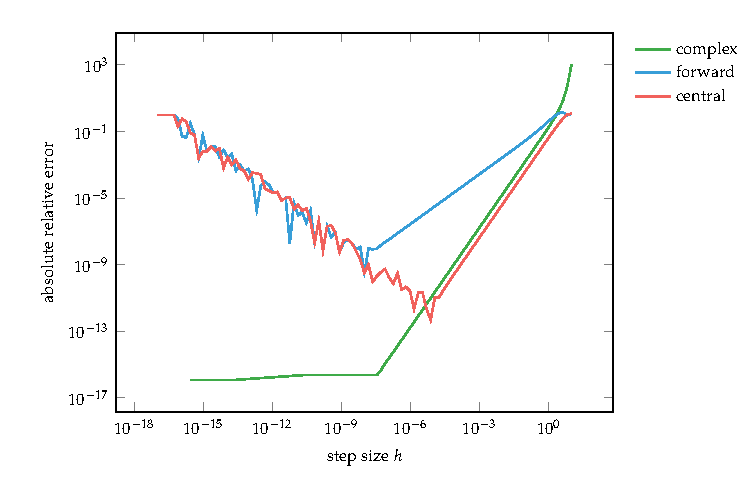
\includegraphics[scale=0.8,page=1]{fig/ndiff.pdf}
  \caption{Evaluation of the numerical derivative of $\sin x$ at $x = \frac{1}{2}$ via different schemes as the step size $h$ is varied.}
\end{figure}

\newpage

\section*{Automatic Differentiation (AD)}

\begin{itemize}
  \item No round-off errors in numerical differentiation
  \item NOT symbolic differentiation of computer algebra systems
  \item Every computer calculation executes a sequence of elementary arithmetic operations ($+$, $-$, $\times$, $\div$, composite) and elementary functions (e.g. $\exp$, $\log$, $\sin$, $\cos$, etc.). 
  \item Applying the chain rule repeatedly; partial derivatives of arbitrary order can be computed automatically
  \item Accurately to working precision, and using at most a small constant factor of more arithmetic operations than the original program
  \item Indispensable for modern applications, many implementations: e.g. \href{https://github.com/HIPS/autograd}{{\tt autograd}}, \href{https://github.com/google/jax}{{\tt JAX}}
  \item Two modes: forward and reverse
  \item \href{https://jingnanshi.com/blog/autodiff.html}{Blog post about fine points of AD and implementations}
  \item References: \citet{naumann,griewank}
\end{itemize}

\newpage

\section*{AD: Forward Mode}

\begin{ex}
  Given $\ds z = x_1 x_2 + \sin x_1$, compute $\ds\frac{\partial z}{\partial x_1}$ at $x_1 = 1.5$, $x_2 = 0.5$.
\end{ex}

\begin{sol}
  \leavevmode
  \vspace{3mm}
  \begin{center}
    \begin{tabular}{ccll}
      \toprule
      Intermediate Var. & Expression & Value & Derivative \\
      \midrule
      $w_1$ & $x_1$ & $1.5$ & $1$ \\
      $w_2$ & $x_2$ & $0.5$ & $0$ \\
      $w_3$ & $w_1 w_2$ & $0.75$ & $0.5$ \\
      $w_4$ & $\sin w_1$ & $0.9974$ & $0.07$ \\
      $w_5$ & $w_3 + w_4$ & $1.7474$ & $0.57$ \\
      \bottomrule
    \end{tabular}
  \end{center}
  \begin{align*}
    \frac{\partial w_3}{\partial x_1} &= \frac{\partial w_3}{\partial w_1}\frac{\partial w_1}{\partial x_1} + \frac{\partial w_3}{\partial w_2}\frac{\partial w_2}{\partial x_1} = w_2\cdot 1 + w_1\cdot 0 = 0.5 \\
    \frac{\partial w_4}{\partial x_1} &= \frac{\partial w_4}{\partial w_1}\frac{\partial w_1}{\partial x_1} = \cos w_1\cdot 1 = \cos(1.5) = 0.07
  \end{align*}
\end{sol}

\newpage

\begin{ex}[\citet{griewank} pp.5]
  $\ds y = \Big(\sin\frac{x_1}{x_2} + \frac{x_1}{x_2} - e^{x_2}\Big)\cdot\Big(\frac{x_1}{x_2} - e^{x_2}\Big)$, compute $\ds\frac{\partial y}{\partial x_1}$ at $x_1 = 1.5$, $x_2 = 0.5$.
\end{ex}

\begin{sol}
  \leavevmode
  \begin{center}
    \begin{tabular}{cccc}
      \toprule
      Intermediate Var. & Expression & Value & Derivative \\
      \midrule
      $w_1$ & $x_1$ & $1.5$ & $1$ \\
      $w_2$ & $x_2$ & $0.5$ & $0$ \\
      $w_3$ & $\frac{w_1}{w_2}$ & $3$ & $2$ \\
      $w_4$ & $\sin w_3$ & $0.1411$ & $-1.98$ \\
      $w_5$ & $e^{w_2}$ & $1.6487$ & $0$ \\
      $w_6$ & $w_3 - w_5$ & $1.3513$ & $2$ \\
      $w_7$ & $w_4 + w_6$ & $1.4924$ & $0.02$ \\
      $w_8$ & $w_6 w_7$ & $2.0167$ & $3.0118$ \\
      \bottomrule
    \end{tabular}
  \end{center}
  \begin{align*}
    \frac{\partial w_3}{\partial x_1} &= \frac{\partial w_3}{\partial w_1}\frac{\partial w_1}{\partial x_1} + \frac{\partial w_3}{\partial w_2}\frac{\partial w_2}{\partial x_1} = \frac{1}{w_2}\cdot 1 + \frac{-w_1}{w_2^2}\cdot 0 = \frac{1}{w_2} = \frac{1}{0.5} = 2 \\
    \frac{\partial w_4}{\partial x_1} &= \frac{\partial w_4}{\partial w_3}\frac{\partial w_3}{\partial x_1} = \cos w_3\cdot\frac{1}{w_2} = \frac{\cos 3}{0.5} = \frac{-0.99}{0.5} = -1.98
  \end{align*}
\end{sol}
\newpage

\section*{AD: Reverse Mode}

\begin{ex}
  Given $\ds z = x_1 x_2 + \sin x_1$, compute $\ds\frac{\partial z}{\partial x_1}$ at $x_1 = 1.5$, $x_2 = 0.5$.
\end{ex}

\begin{sol}
  Set 
  \begin{align*}
    w_1 &= x_1 \\
    w_2 &= x_2 \\
    w_3 &= w_1 w_2 \\
    w_4 &= \sin w_1 \\
    w_5 &= w_3 + w_4 \\
    z & = w_5
  \end{align*}
  
  \begin{align*}
    \frac{\partial z}{\partial x_1} &= \frac{\partial z}{\partial w_1} = \frac{\partial w_5}{\partial w_1} = \frac{\partial w_5}{\partial w_3}\frac{\partial w_3}{\partial w_1} + \frac{\partial w_5}{\partial w_4}\frac{\partial w_4}{\partial w_1} \\ &= w_2 + \cos w_1 = 0.5 + \cos(1.5) = 0.5 + 0.07 = 0.57
  \end{align*}
  %$\ds\frac{\partial z}{\partial x_2} = \frac{\partial z}{\partial w_2} = \frac{\partial w_5}{\partial w_2} = \frac{\partial w_5}{\partial w_3}\frac{\partial w_3}{\partial w_2} + \frac{\partial w_5}{\partial w_4}\frac{\partial w_4}{\partial w_2} = 1\cdot w_1 +1\cdot 0 = w_1 = 1.5$. 
\end{sol}

\newpage

\begin{ex}[\citet{griewank} pp.5]
  $\ds y = \Big(\sin\frac{x_1}{x_2} + \frac{x_1}{x_2} - e^{x_2}\Big)\cdot\Big(\frac{x_1}{x_2} - e^{x_2}\Big)$, compute $\ds\frac{\partial y}{\partial x_1}$ at $x_1 = 1.5$, $x_2 = 0.5$.
\end{ex}

\begin{sol}
  Set
  \begin{align*}
    w_1 &= x_1,\quad w_2 = x_2,\quad w_3 = \frac{w_1}{w_2},\quad w_4 = \sin w_3,\quad w_5 = e^{w_2} \\
    w_6 &= w_3 - w_5,\quad w_7 = w_4 + w_6,\quad w_8 = w_6\cdot w_7,\quad y = w_8
  \end{align*}
  $\ds\frac{\partial y}{\partial x_1} = \frac{\partial y}{\partial w_1} = \frac{\partial w_8}{\partial w_1} = \frac{\partial w_8}{\partial w_6}\frac{\partial w_6}{\partial w_1} + \frac{\partial w_8}{\partial w_7}\frac{\partial w_7}{\partial w_1} = w_7\frac{\partial w_6}{\partial w_1} + w_6\frac{\partial w_7}{\partial w_1} \\= w_7\frac{\partial w_6}{\partial w_1} + w_6\Big(\frac{\partial w_4}{\partial w_1} + \frac{\partial w_6}{\partial w_1}\Big) = (w_7 + w_6)\Big(\frac{\partial w_3}{\partial w_1} - \frac{\partial w_5}{\partial w_1}\Big) + w_6\Big(\frac{\partial w_4}{\partial w_1}\Big) \\= (w_7 + w_6)\frac{\partial w_3}{\partial w_1} + w_6\frac{\partial w_4}{\partial w_3}\frac{\partial w_3}{\partial w_1} = (w_7 + w_6(1 + \cos w_3))\frac{\partial w_3}{\partial w_1} \\= \frac{w_7 + w_6(1 + \cos w_3)}{w_2}$. Now $w_1 = x_1 = 1.5$, $w_2 = x_2 = 0.5$, $w_3 = 3$, $w_4 = 0.1411$, $w_5 = 1.6487$, $w_6 = 3 - 1.6487 = 1.3513$, $w_7 = 0.1411 + 1.3513 = 1.4924$, so $\ds\frac{\partial y}{\partial x_1} = \frac{1.4924 + 1.3513\cdot(1 + \cos 3)}{0.5} = 3.0118$. ($\cos 3 = -0.99$)
\end{sol}

\newpage

\section*{Choosing Forward / Reverse Mode}

\begin{itemize}\setlength\itemsep{0em}
  \item The chain rule: the Jacobian of a operation is the matrix multiplication of all the Jacobians of sub-operations
  %\item The difference between forward and reverse mode of AD is the \emph{order} in which one multiply those Jacobians
  \item Let $\ds\vy = f(\vx) = r(q(p(\vx)))$ and $\va = p(\vx)$, $\vb = q(\va)$, $y = r(\vb)$; the Jacobian reads
    \begin{align*}
      \underbrace{\frac{\partial\vy}{\partial\vx}}_{|\vy|\times|\vx|} = \underbrace{\frac{\partial r(\vb)}{\partial\vb}}_{|\vy|\times|\vb|}\,\underbrace{\frac{\partial q(\va)}{\partial\va}}_{|\vb|\times|\va|}\,\underbrace{\frac{\partial p(\vx)}{\partial\vx}}_{|\va|\times|\vx|}
    \end{align*}
  \item The number of scalar multiplications required to multiply two matrices of sizes $\alpha\times\beta$ and $\beta\times\gamma$ is $\alpha\cdot\beta\cdot\gamma$
  \item Forward mode: $\ds\frac{\partial\vy}{\partial\vx} = \frac{\partial r(\vb)}{\partial\vb}\,\Big(\frac{\partial q(\va)}{\partial\va}\,\frac{\partial p(\vx)}{\partial\vx}\Big)$, $\;\ds|\vb|\cdot|\va|\cdot|\vx| + |\vy|\cdot|\vb|\cdot|\vx|$ multiplications
  \item Reverse mode: $\ds\frac{\partial\vy}{\partial\vx} = \Big(\frac{\partial r(\vb)}{\partial\vb}\,\frac{\partial q(\va)}{\partial\va}\Big)\,\frac{\partial p(\vx)}{\partial\vx}$, $\;\ds|\vy|\cdot|\vb|\cdot|\va| + |\vy|\cdot|\va|\cdot|\vx|$ multiplications
  \item Assume $|\va| = |\vb|$. If $|\vy| > |\vx|$, forward mode involves fewer steps; else if $|\vy| < |\vx|$, reverse mode involves fewer steps
\end{itemize}

\newpage

\bibliographystyle{elsarticle-harv}
\bibliography{note04}

\end{document}
